\documentclass[tikz,border=5pt]{standalone}
\usetikzlibrary{spath3}
\begin{document}
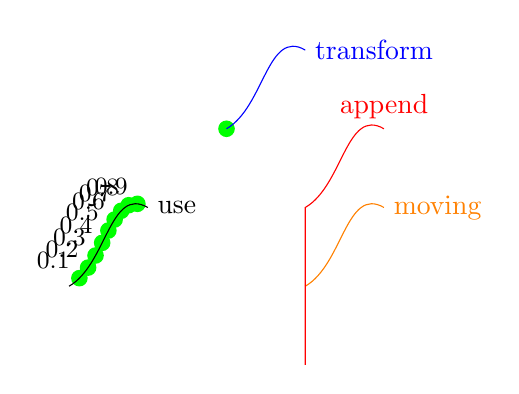
\begin{tikzpicture}
    \path[spath/save=rpath] (0,0) to[out=30,in=150] (1,1); 
    \foreach \k in {1,...,9} {
        \fill[green] (spath cs:rpath 0.\k) circle[radius=3pt] node[above left,text=black,font=\small] {\(0.\k\)};
    }

    \fill[green] (2,2) circle[radius=3pt];
    \draw[blue, spath/transform={rpath}{shift={(2,2)}},spath/use=rpath] node[right] {transform};

    \draw[orange] (3,0) [spath/use={rpath, move}] node[right] {moving};

    \draw[red] (3,-1) -- +(0,2) [spath/append=rpath] node[above]
    {append};

    \draw[spath/use=rpath] node[right] {use};
\end{tikzpicture}
\end{document}